\documentclass[a0,plainsections,30pt]{sciposter}\usepackage[]{graphicx}\usepackage[]{color}
%% maxwidth is the original width if it is less than linewidth
%% otherwise use linewidth (to make sure the graphics do not exceed the margin)
\makeatletter
\def\maxwidth{ %
  \ifdim\Gin@nat@width>\linewidth
    \linewidth
  \else
    \Gin@nat@width
  \fi
}
\makeatother

\definecolor{fgcolor}{rgb}{0.345, 0.345, 0.345}
\newcommand{\hlnum}[1]{\textcolor[rgb]{0.686,0.059,0.569}{#1}}%
\newcommand{\hlstr}[1]{\textcolor[rgb]{0.192,0.494,0.8}{#1}}%
\newcommand{\hlcom}[1]{\textcolor[rgb]{0.678,0.584,0.686}{\textit{#1}}}%
\newcommand{\hlopt}[1]{\textcolor[rgb]{0,0,0}{#1}}%
\newcommand{\hlstd}[1]{\textcolor[rgb]{0.345,0.345,0.345}{#1}}%
\newcommand{\hlkwa}[1]{\textcolor[rgb]{0.161,0.373,0.58}{\textbf{#1}}}%
\newcommand{\hlkwb}[1]{\textcolor[rgb]{0.69,0.353,0.396}{#1}}%
\newcommand{\hlkwc}[1]{\textcolor[rgb]{0.333,0.667,0.333}{#1}}%
\newcommand{\hlkwd}[1]{\textcolor[rgb]{0.737,0.353,0.396}{\textbf{#1}}}%
\let\hlipl\hlkwb

\usepackage{framed}
\makeatletter
\newenvironment{kframe}{%
 \def\at@end@of@kframe{}%
 \ifinner\ifhmode%
  \def\at@end@of@kframe{\end{minipage}}%
  \begin{minipage}{\columnwidth}%
 \fi\fi%
 \def\FrameCommand##1{\hskip\@totalleftmargin \hskip-\fboxsep
 \colorbox{shadecolor}{##1}\hskip-\fboxsep
     % There is no \\@totalrightmargin, so:
     \hskip-\linewidth \hskip-\@totalleftmargin \hskip\columnwidth}%
 \MakeFramed {\advance\hsize-\width
   \@totalleftmargin\z@ \linewidth\hsize
   \@setminipage}}%
 {\par\unskip\endMakeFramed%
 \at@end@of@kframe}
\makeatother

\definecolor{shadecolor}{rgb}{.97, .97, .97}
\definecolor{messagecolor}{rgb}{0, 0, 0}
\definecolor{warningcolor}{rgb}{1, 0, 1}
\definecolor{errorcolor}{rgb}{1, 0, 0}
\newenvironment{knitrout}{}{} % an empty environment to be redefined in TeX

\usepackage{alltt}

\usepackage{graphicx}
\usepackage{amsmath}
\usepackage{amsthm}
\usepackage{amssymb}
\usepackage{bbm}
\usepackage{natbib}

\setlength{\columnseprule}{0pt}

\newcommand{\Expect}{\mathbb{E}}
\newcommand{\etaopt}{\eta^{*}}

\newcommand{\targetexpectation}{\Expect_{q_{\eta^*}}
\left[\#\{\substack{\text{distinct clusters}\\\text{in new dataset}}\} \right]}

\usepackage[framemethod=TikZ, xcolor=RGB]{mdframed}

\definecolor{mydarkblue}{rgb}{0,.06,.5}
\definecolor{mydarkred}{rgb}{.5,0,.1}
\definecolor{myroyalblue}{rgb}{0,.1,.8}

\usepackage{sectsty}
\sectionfont{\color{mydarkblue}\centering\LARGE\bf}

\mdfdefinestyle{MyFrame}{%
    linecolor=mydarkblue,
    outerlinewidth=2pt,
    roundcorner=20pt,
    innertopmargin=10pt,
    innerbottommargin=10pt,
    innerrightmargin=10pt,
    innerleftmargin=10pt,
    backgroundcolor=blue!10}


\title{\textcolor{mydarkblue}{
Evaluating Sensitivity to the Stick Breaking Prior in Bayesian Nonparametrics
}}

\author{%
Runjing Liu\textsuperscript{1*} \quad
Ryan Giordano\textsuperscript{2*} \quad
Michael I. Jordan\textsuperscript{1} \quad
Tamara Broderick\textsuperscript{2} \\
{\large\normalfont
 \textsuperscript{1}Department of Statistics, UC Berkeley\quad
 \textsuperscript{2}CSAIL, MIT\quad
 \textsuperscript{*}Equal contribution authors}
}

\leftlogo[1]{static_images/logo_left.png}
\rightlogo[1]{static_images/faces.jpg}

% Fiddle with the margin
\addtolength{\topmargin}{-0.5in}
\addtolength{\textheight}{1in}
\IfFileExists{upquote.sty}{\usepackage{upquote}}{}
\begin{document}
\conference{BNP 2019}

\setlength{\parskip}{0.25em}

\maketitle

\vspace{-1in}




%%%%%%%%%%%%%%%%%%%%%%%%%%%%%%%%%
%%%%%%%%%%%%%%%%%%%%%%%%%%%%%%%%%
% FIRST COLUMN
%%%%%%%%%%%%%%%%%%%%%%%%%%%%%%%%%
%%%%%%%%%%%%%%%%%%%%%%%%%%%%%%%%%

\begin{minipage}[t]{0.45\textwidth}

\begin{mdframed}[style=MyFrame]
%%%%%%%%%%%%%%%%%%%%%%%%%%%%%%%%%
%%%%%%%%%%%%%%%%%%%
\section*{Overview}
\vspace{-0.3in}
%%%%%%%%%%%%%%%%%%%
%%%%%%%%%%%%%%%%%%%%%%%%%%%%%%%%%
\begin{itemize}
\item Researchers often want to estimate the number of distinct clusters
that would be present in a new dataset.

\item A variational Bayes (VB) approximation to a Bayesian nonparametric (BNP)
model makes inferring the number of clusters amenable to Bayesian inference.
%We approximate the exact posterior with variational Bayes (VB).

\item \textbf{Question}: How sensitive are the
VB approximation and the resulting inference to BNP model choices?

\item \textbf{Problem}: Re-running VB for multiple model choices is expensive.

\item \textbf{We propose}: A local approximation to efficiently
estimate BNP sensitivity from a single run of VB, avoiding
expensive refitting.

%\item We evaluate sensitivity to parametric and functional perturbations.
\end{itemize}
\end{mdframed}
\vspace{-0.7in}

%%%%%%%%%%%%%%%%%%%%%%%%%%%%%%%%%
%%%%%%%%%%%%%%%%%%%%%%%%%%%%%%%%%
\section*{Model and inference }
\vspace{-0.3in}
%%%%%%%%%%%%%%%%%%%%%%%%%%%%%%%%%
%%%%%%%%%%%%%%%%%%%%%%%%%%%%%%%%%

The \textbf{Dirichlet process} is a popular Bayesian nonparametric
(BNP) model used for clustering.  A stick-breaking representation uses
a distribution on sticks $\{\nu_k\}$ to induce a prior on component
probabilities $\{\pi_k\}$.

\begin{figure}
\centering
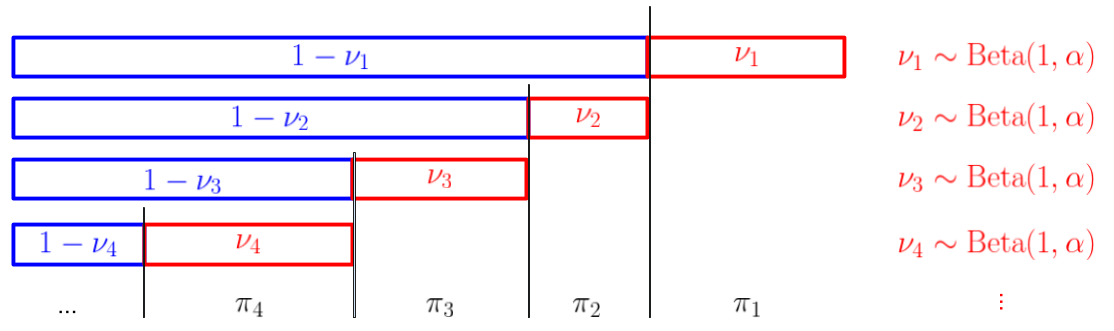
\includegraphics[width = 0.95\textwidth]{./static_images/DP_stick_breaking.png}
\caption{The Dirichlet stick-breaking process with $\nu_k \sim \mathrm{Beta}(1, \alpha)$.}
\end{figure}
%
\vspace{-0.3in}
Define:
\begin{itemize}
\item $\epsilon :=$ Any real-valued hyperparameter for the stick-breaking prior
    $p(\nu_k | \epsilon)$.
\item $\etaopt :=$ The optimal variational parameters.
\item $\targetexpectation :=$ The quantity we want to infer.
\end{itemize}

\begin{mdframed}[style=MyFrame]
VB inference defines a map:
%
\begin{gather*}
\textrm{Stick-breaking prior}
    \mapsto \textrm{VB approximation}
    \mapsto \textrm{Posterior expected \# clusters},\\
\textrm{i.e.,}\\
\epsilon
    \mapsto \etaopt
    \mapsto \targetexpectation.
\end{gather*}
\end{mdframed}

%%%%%%%%%%%%%%%%%%%%%%%%%%%%%%%%%
%%%%%%%%%%%%%%%%%%%%%%%%%

\textbf{Parametric perturbation.} To stay within the class of Dirichlet
processes, we might take $\epsilon := \alpha - \alpha_0$ and $p(\nu_k | \alpha) :=
\mathrm{Beta}(\nu_k | 1, \alpha)$.

\textbf{Functional perturbation.} Suppose we are interested in the effect of
replacing the original beta prior $p_0(\nu_k) := \mathrm{Beta}(\nu_k | 1,
\alpha)$ with another distribution $p_1(\nu_k)$. Then we take $\epsilon :=
\delta$ in
%
\vspace{-0.3in}
\begin{align*}
p(\nu_k \vert \delta) \propto
    p_{0}(\nu_k)\left(\frac{p_1(\nu_k)}{p_0(\nu_k)}\right)^\delta.
\end{align*}
\vspace{-0.3in}

By using a multiplicative perturbation, the map $p_1 \mapsto \etaopt$ is
Fr\'{e}chet differentiable in the norm $\left\Vert p_1 / p_0
\right\Vert_\infty$.

%%%%%%%%%%%%%%%%%%%%%%%%%%%%%%%%%
%%%%%%%%%%%%%%%%%%%%%%%%%
\vspace{-0.3in}
\subsection*{Local approximation to dependence on the prior}
\vspace{-0.2in}
%%%%%%%%%%%%%%%%%%%%%%%%%
%%%%%%%%%%%%%%%%%%%%%%%%%%%%%%%%%
Let $\epsilon=0$ represent the original prior at which we fit a VB
approximation.

\begin{mdframed}[style=MyFrame]
For any other $\epsilon \ne 0$ we approximate $\epsilon \mapsto \etaopt$ with
\begin{align*}
\eta^*(\epsilon)  &\approx  \eta^*(0) +
\frac{d \eta^*(\epsilon)}{d\epsilon^T}\Big|_{\epsilon=0} \epsilon.
\end{align*}
We retain the non-linearities in $\etaopt \mapsto \targetexpectation$.
\end{mdframed}

\begin{itemize}
\item We can \textbf{automatically compute}
    the local approximation
    using automatic differentiation \cite{giordano:2017:covariances}.
    %\cite{giordano:2017:covariances, maclaurin:2015:autograd}.
\item The approximation requires the
    \textbf{inverse Hessian of the VB objective}.
\item This is an application of \textbf{local Bayesian robustness}
\citep{gustafson:1996:localposterior}.
\end{itemize}

\end{minipage}
\hfill \vrule \hfill
\begin{minipage}[t]{0.45\textwidth}

%%%%%%%%%%%%%%%%%%%%%%%%%%%%%%%%%
%%%%%%%%%%%%%%%%%%%%%%%%%%%%%%%%%
% SECOND COLUMN
%%%%%%%%%%%%%%%%%%%%%%%%%%%%%%%%%
%%%%%%%%%%%%%%%%%%%%%%%%%%%%%%%%%



%%%%%%%%%%%%%%%%%%%%%%%%%%%%%%%%%
%%%%%%%%%%%%%%%%%%
\section*{Data}
\vspace{-0.3in}
%
\begin{minipage}[t]{0.49\textwidth}
%
\textbf{Iris data.}
For our first dataset, we discard species
information and cluster the 150 four-dimensional observations of the Fisher iris
dataset \citep{iris_data_anderson}.
The loadings on the first two principal components are shown
to the right.
%
\end{minipage}
%
\begin{minipage}[t]{0.49\textwidth}

%
\vspace{-0.4in}
\begin{knitrout}
\definecolor{shadecolor}{rgb}{0.969, 0.969, 0.969}\color{fgcolor}

{\centering 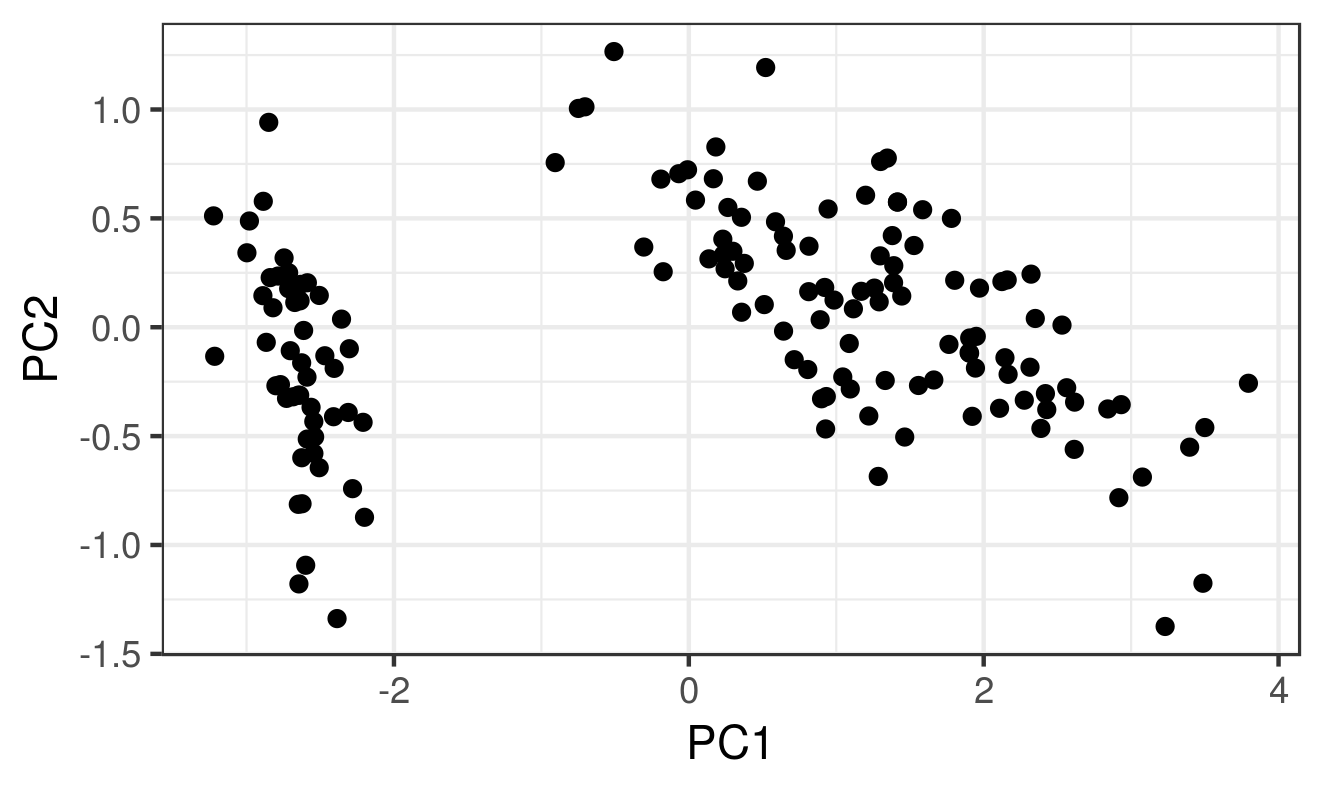
\includegraphics[width=0.98\linewidth,height=0.588\linewidth]{figure/iris_pca-1} 

}



\end{knitrout}
\end{minipage}
%

\vspace{1em}

\begin{minipage}[t]{0.49\textwidth}
%
\textbf{Mouse data.} For our second dataset, we use a publicly available
dataset of gene expression in mice \citep{shoemaker:2015:ultrasensitive}. We
smooth and center 7000 gene expression time series and cluster the resulting
patterns.  A typical smoothed time series is shown to the right.  The faint
lines show regression posterior uncertainty.
%
\end{minipage}
%
\begin{minipage}[t]{0.49\textwidth}
\vspace{-0.8in}
\begin{figure}[!h]
\centering
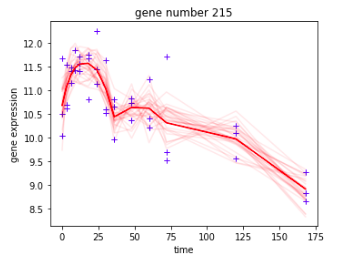
\includegraphics[width = 0.95\textwidth]{./static_images/mouse_genes.png}
\end{figure}
\end{minipage}
%

%%%%%%%%%%%%%%%%%%%%%%%%%%%%%%%%%
%%%%%%%%%%%%%%%%%%
\vspace{-0.6in}
\section*{Results}
\vspace{-0.3in}

\textbf{Parametric perturbation.} Vertical lines show the location of
$\alpha_0$.
\begin{itemize}
\item VB + BNP is robust for the mouse data but not the iris data.
\item The approximation \textbf{extrapolates best from more to fewer clusters.}
\end{itemize}

\vspace{0.05in}
%

\begin{knitrout}
\definecolor{shadecolor}{rgb}{0.969, 0.969, 0.969}\color{fgcolor}

{\centering 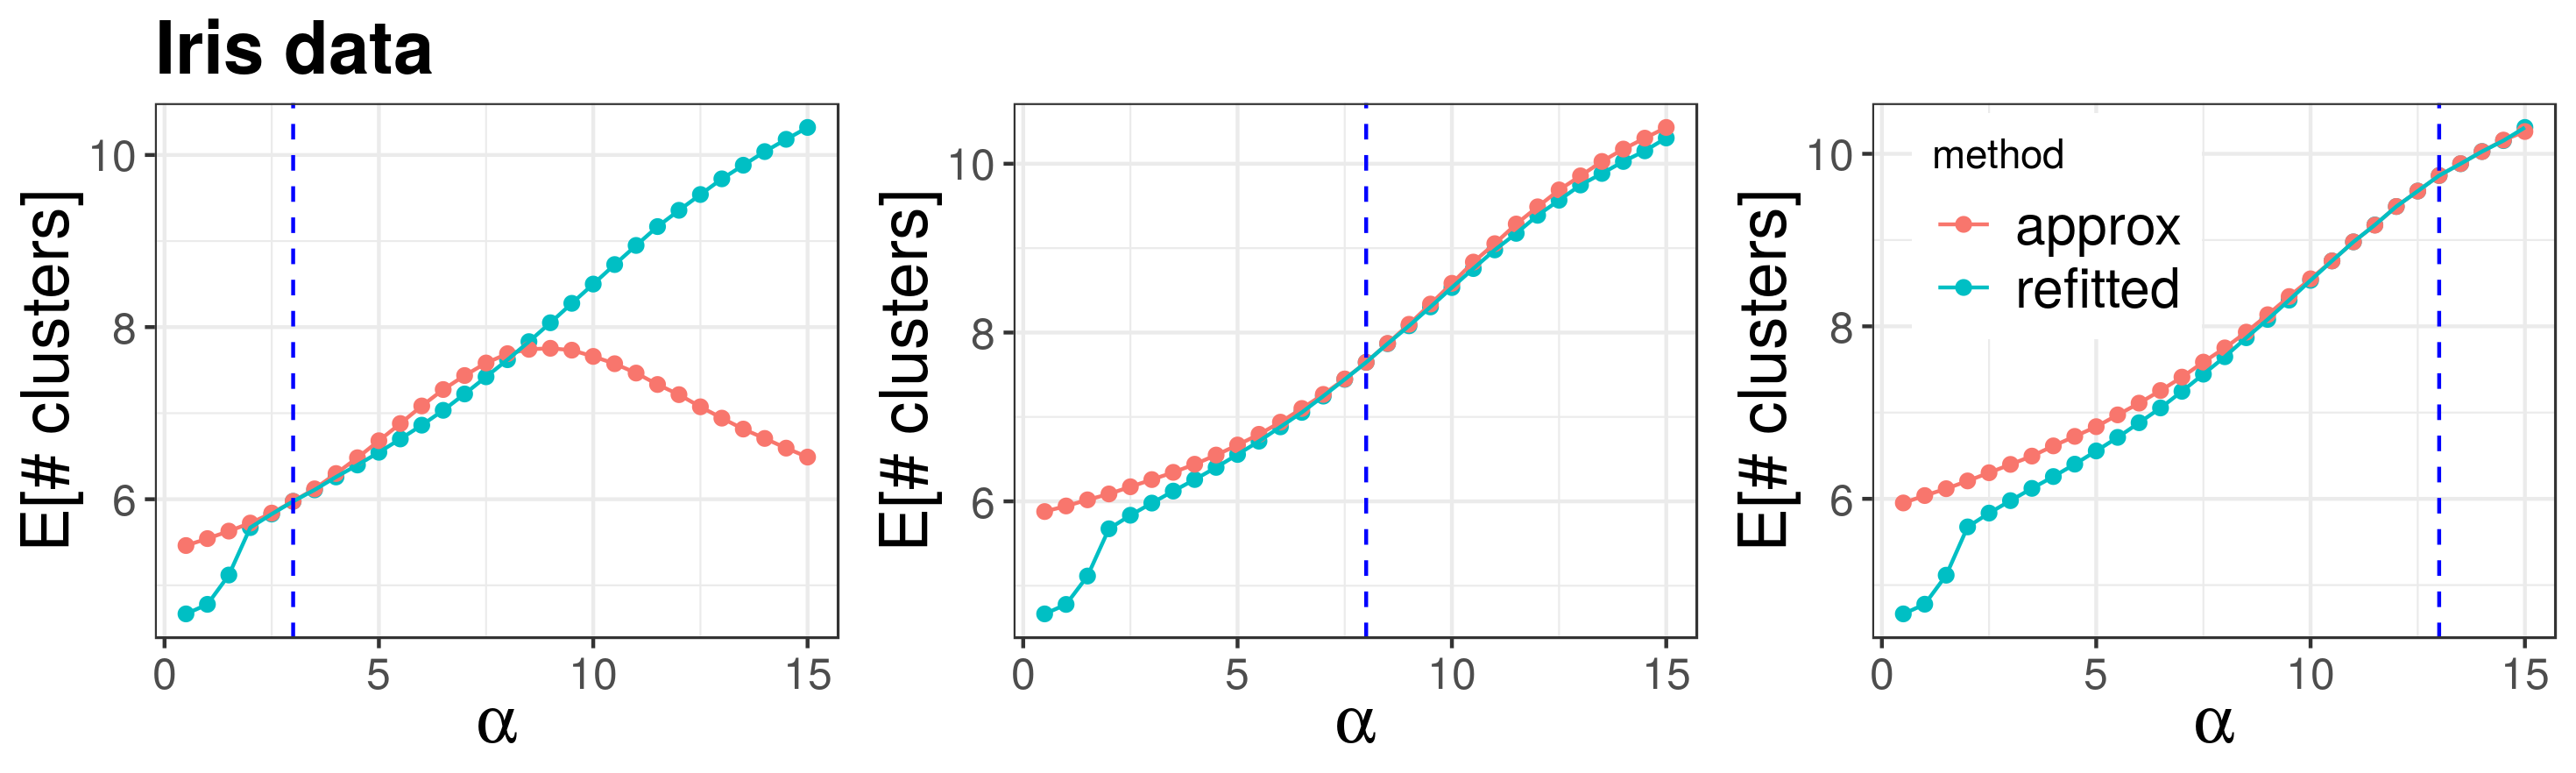
\includegraphics[width=0.98\linewidth,height=0.294\linewidth]{figure/param_sens_plot-1} 

}



\end{knitrout}

\begin{knitrout}
\definecolor{shadecolor}{rgb}{0.969, 0.969, 0.969}\color{fgcolor}

{\centering 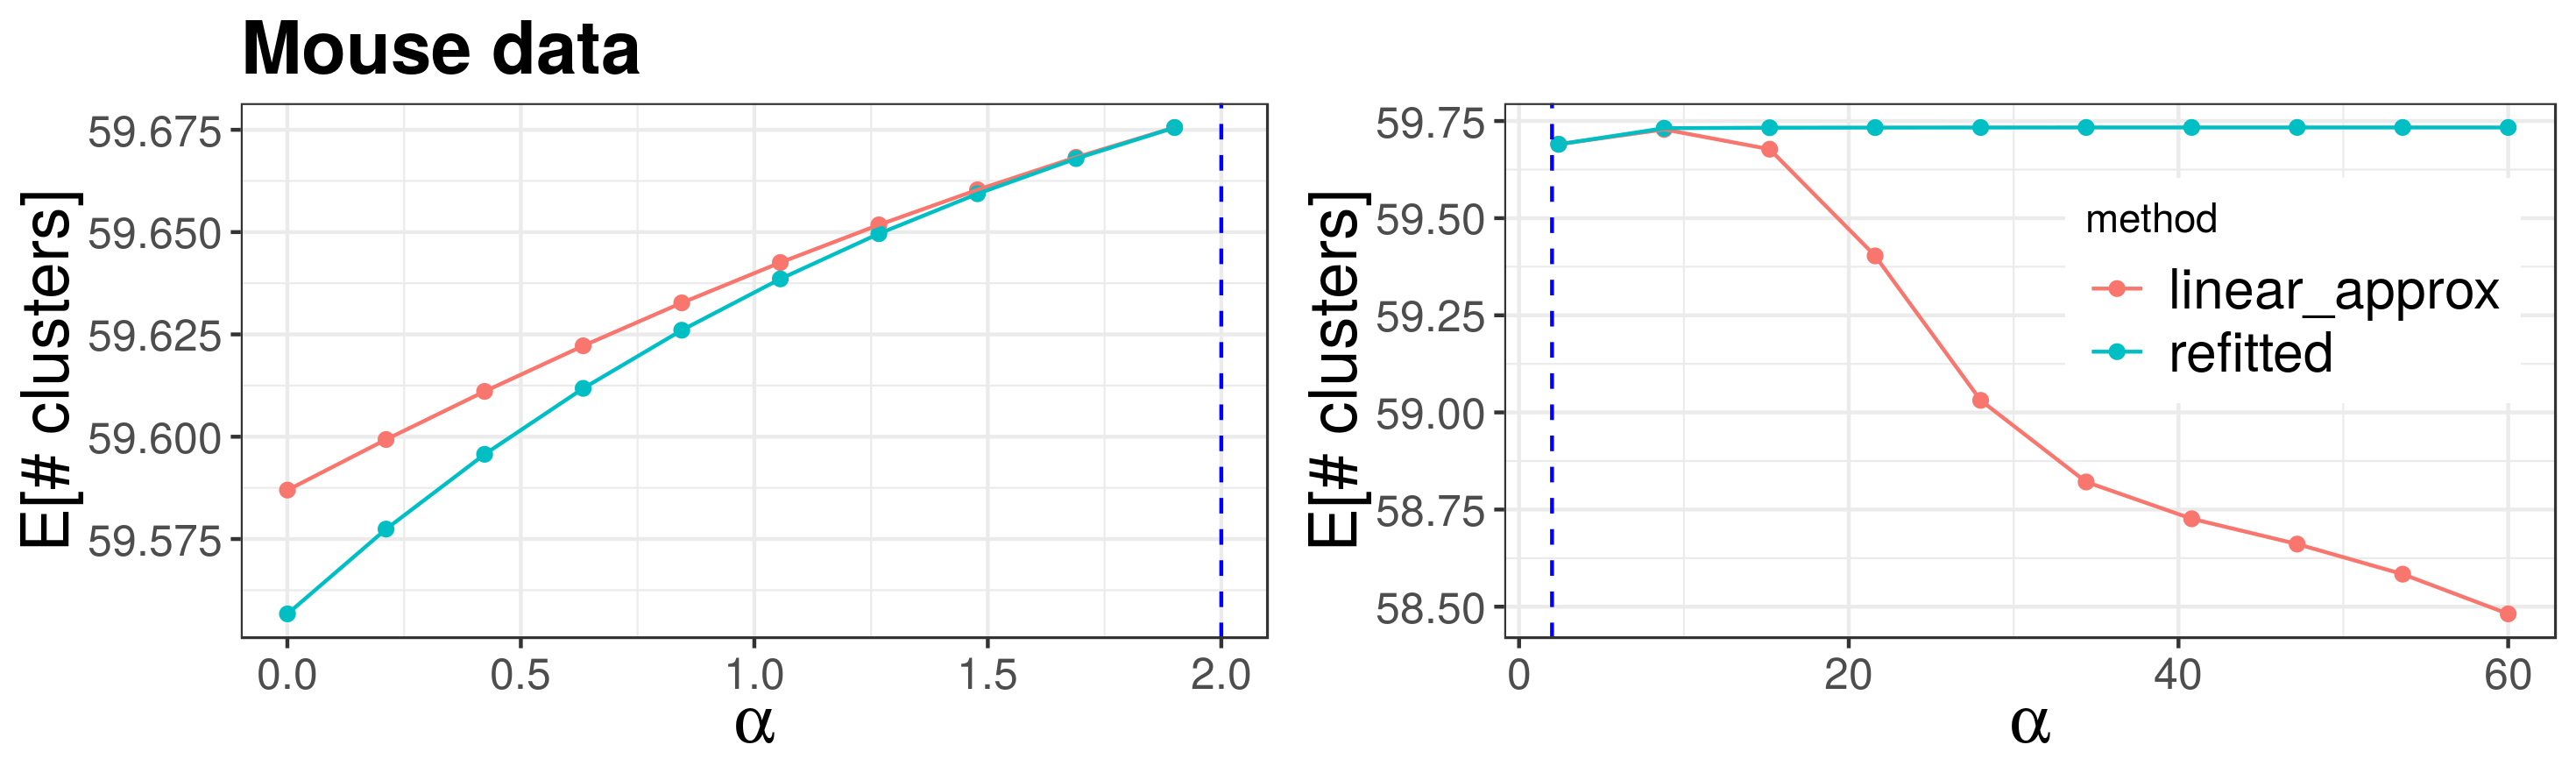
\includegraphics[width=0.98\linewidth,height=0.294\linewidth]{figure/gene_param_sens_plot-1} 

}



\end{knitrout}

\textbf{Functional perturbation.} The first row shows the original prior
$p_0(\nu_k)$ and the functional perturbation $p_1(\nu_k)$.  Again, VB + BNP
is robust for the mouse data but not the iris data, and the approximation
extrapolates best from more to fewer clusters.

\vspace{0.1in}

\begin{knitrout}
\definecolor{shadecolor}{rgb}{0.969, 0.969, 0.969}\color{fgcolor}

{\centering 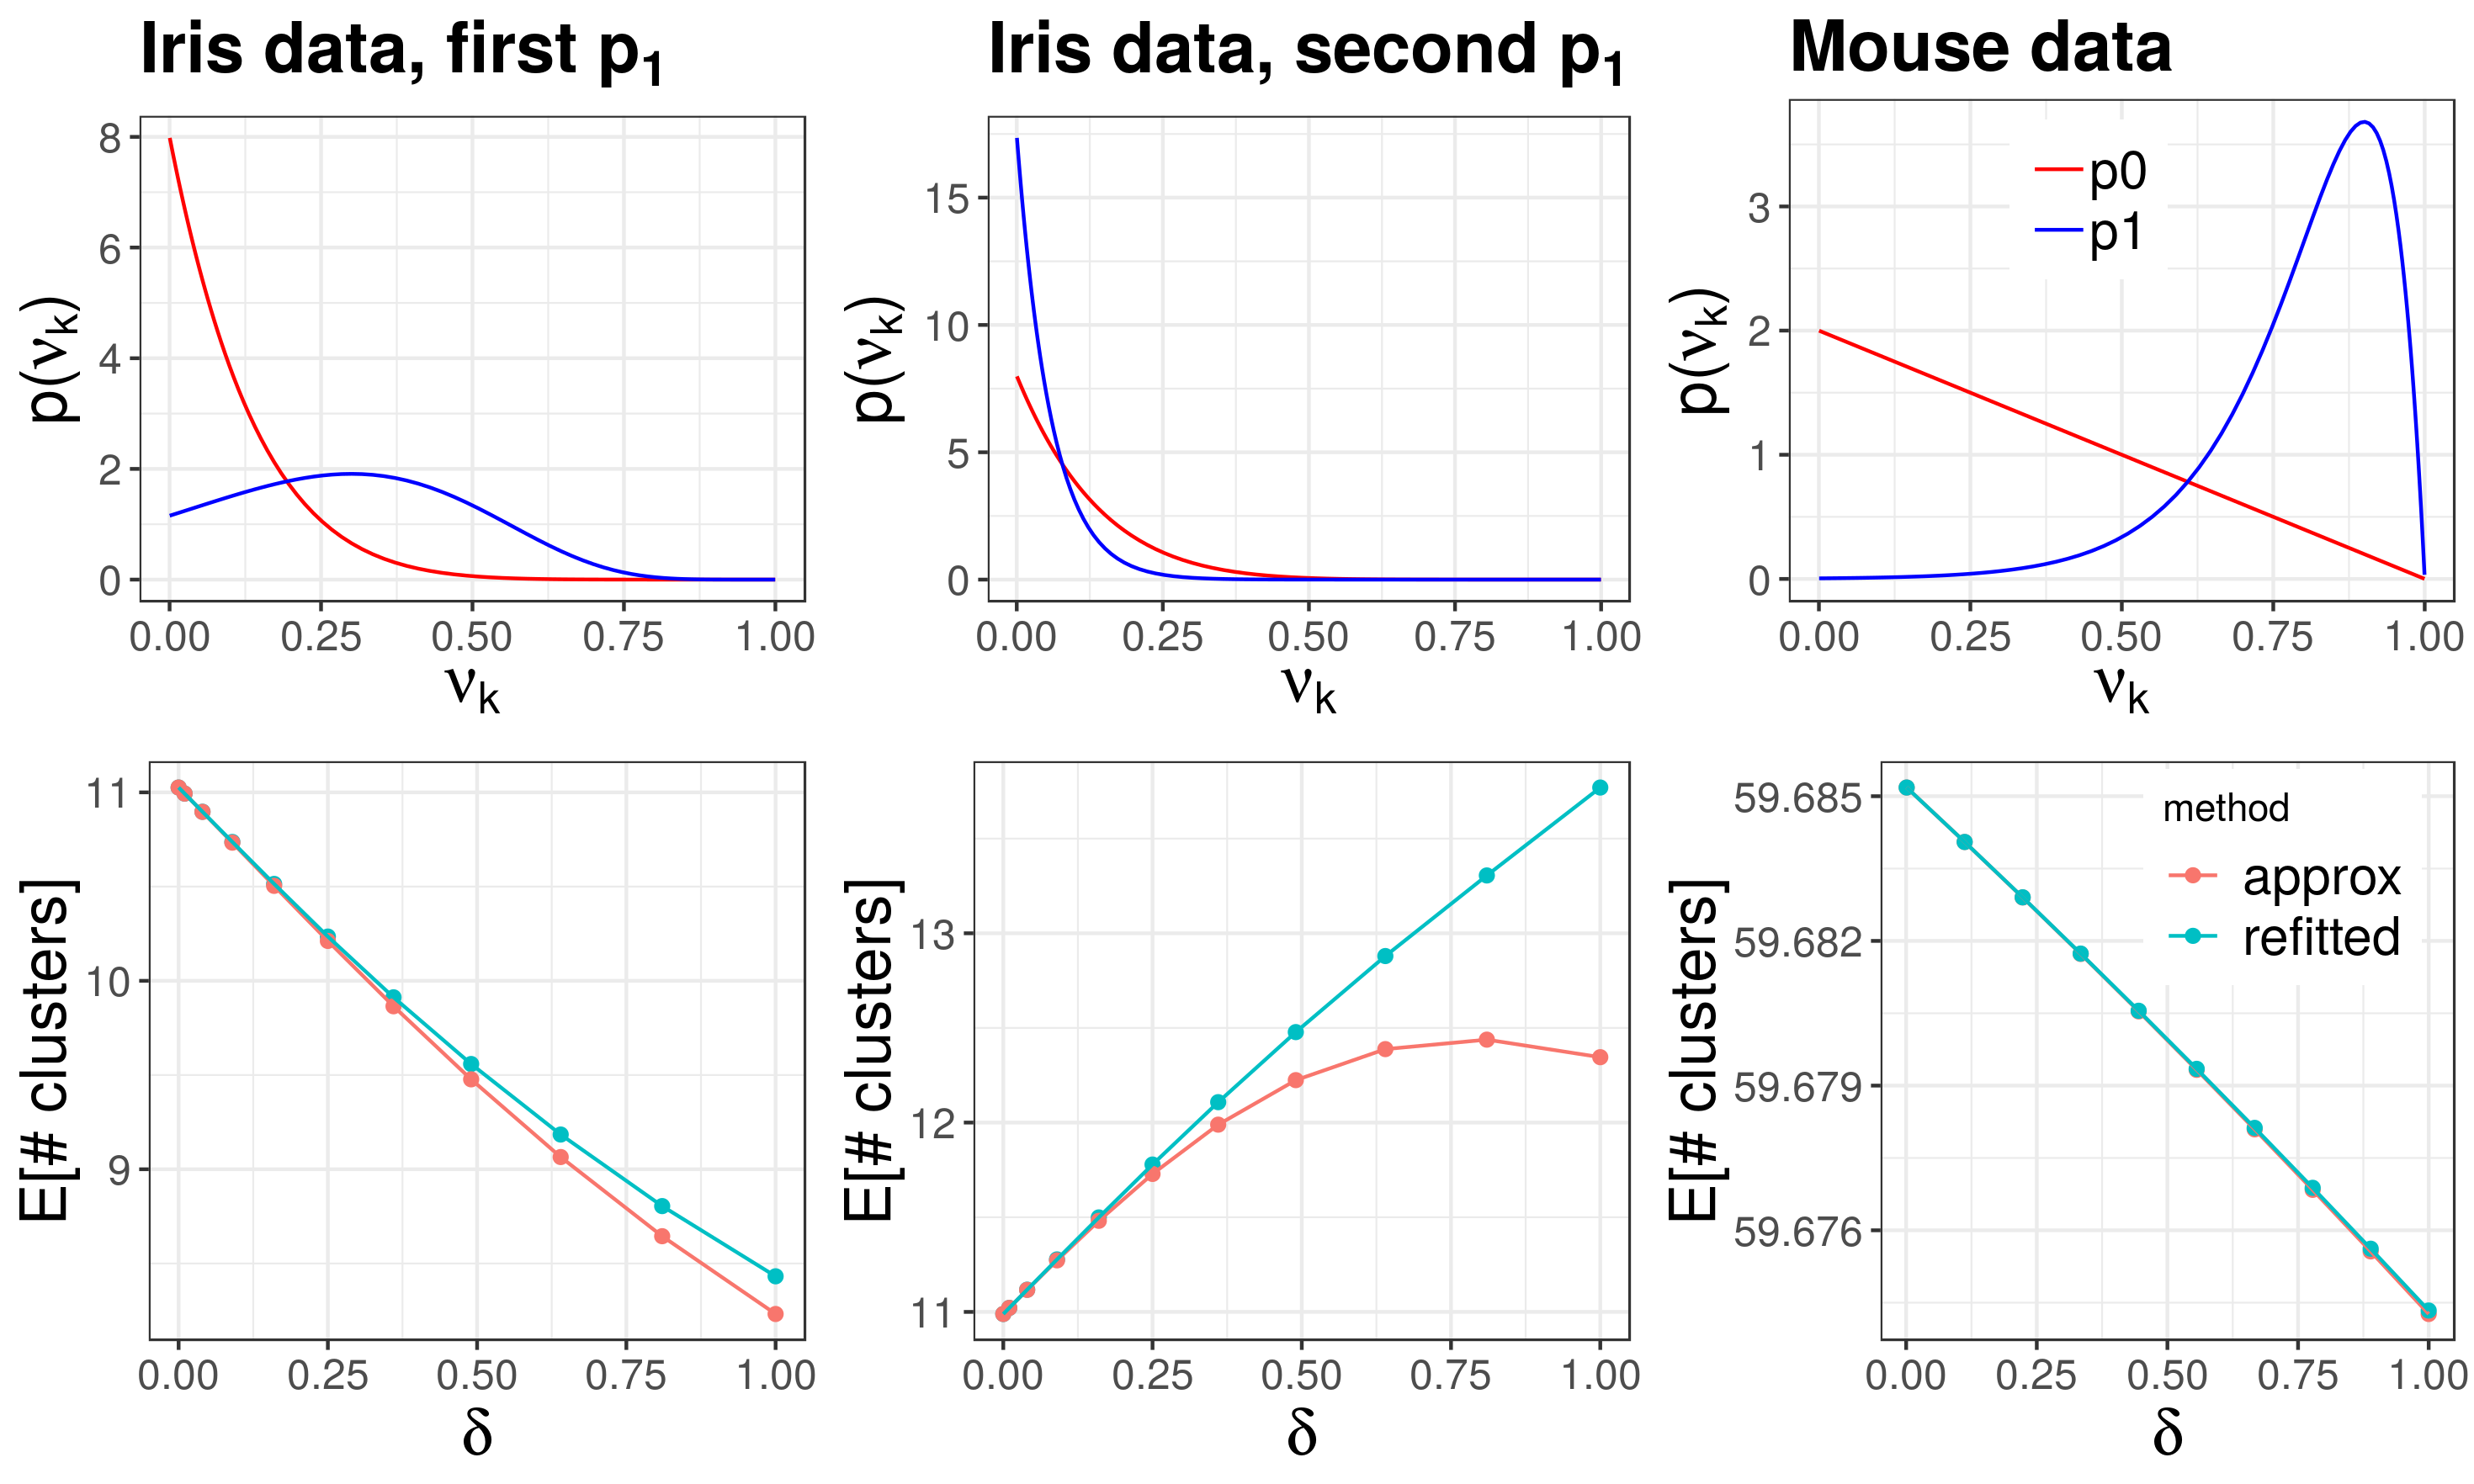
\includegraphics[width=0.98\linewidth,height=0.588\linewidth]{figure/functional_sens_plot-1} 

}



\end{knitrout}

\noindent\rule{0.95\textwidth}{1pt}

\textbf{Contact and code:} rgiordan@mit.edu, runjing\_liu@berkeley.edu
{\color{blue} https://github.com/Runjing-Liu120/sensitivity\_to\_stick\_breaking\_in\_BNP}
{\color{blue} https://github.com/rgiordan/vittles}
(sensitivity analysis)

\end{minipage}\\

\begin{center}
\noindent\rule{0.95\textwidth}{1pt}
\end{center}

\small{
%%%%%%%%%%%%%%%%%%%%%%%%%%%%%%%
%%%%%%%%%%%%%%%%%
{\bf Acknowledgments}:
% %%%%%%%%%%%%%%%%%%
%%%%%%%%%%%%%%%%%%%%%%%%%%%%%%%%%
Ryan Giordano's research was funded in full by the
Gordon and Betty Moore Foundation through Grant GBMF3834 and by the Alfred P. Sloan Foundation through Grant 2013-10-27 to the University of California, Berkeley. Runjing Liu's research was funded by the NSF graduate research fellowship. Tamara Broderick's research is supported by an NSF CAREER Award and an ARO YIP
Award. This research is supported in part by the DARPA program on
Lifelong Learning Machines.
}


\renewcommand{\section}[2]{}%
\footnotesize{
  \bibliographystyle{abbrv}
  \bibliography{./references}
}

\end{document}
